\documentclass[b5paper,papersize,twoside,dvipdfmx]{jsarticle}
\pagestyle{headings}
\usepackage{After}
\usepackage{url}
\usepackage{graphicx}
\begin{document}
% 中央揃えで大きな文字にする部分
\begin{center}
\Large 4302 東瑛太郎
\end{center}
\section{はじめにー自己紹介ー}
こんにちは! この度第65代物理部部長に就任した東です。この代は基本的に有能な人が多くて、みんな一つくらい特別な技術を持ってたりするんですが、僕は中一から物理部で活動していながら配線くらいしか取り柄がないです...

けど物理部は大好きなのでみんなをサポートしながら一年間頑張っていきたいと思います。目指せ参団グランプリ総合1位!!
\section{作品}
\subsection{ラジコン船}
現在高一の楊康弘・中嶋幹・東の三人で制作しました。ここでは文化祭直前に完成した船「M4」を、プログラム・設計(3Dモデリング)・その他に分けて説明します。
\subsubsection{プログラム}
詳しい説明をしようとすると煩雑になるので、GitHubのソースコードを共有します。
\url{https://github.com/motokisama/remote-controller}

このリポジトリにはArduinoとラズパイ、それから陸上の制御用PCのコードが入っています。それぞれの機器の配線は以下のようになります。
\begin{figure}[htbp]
\centering
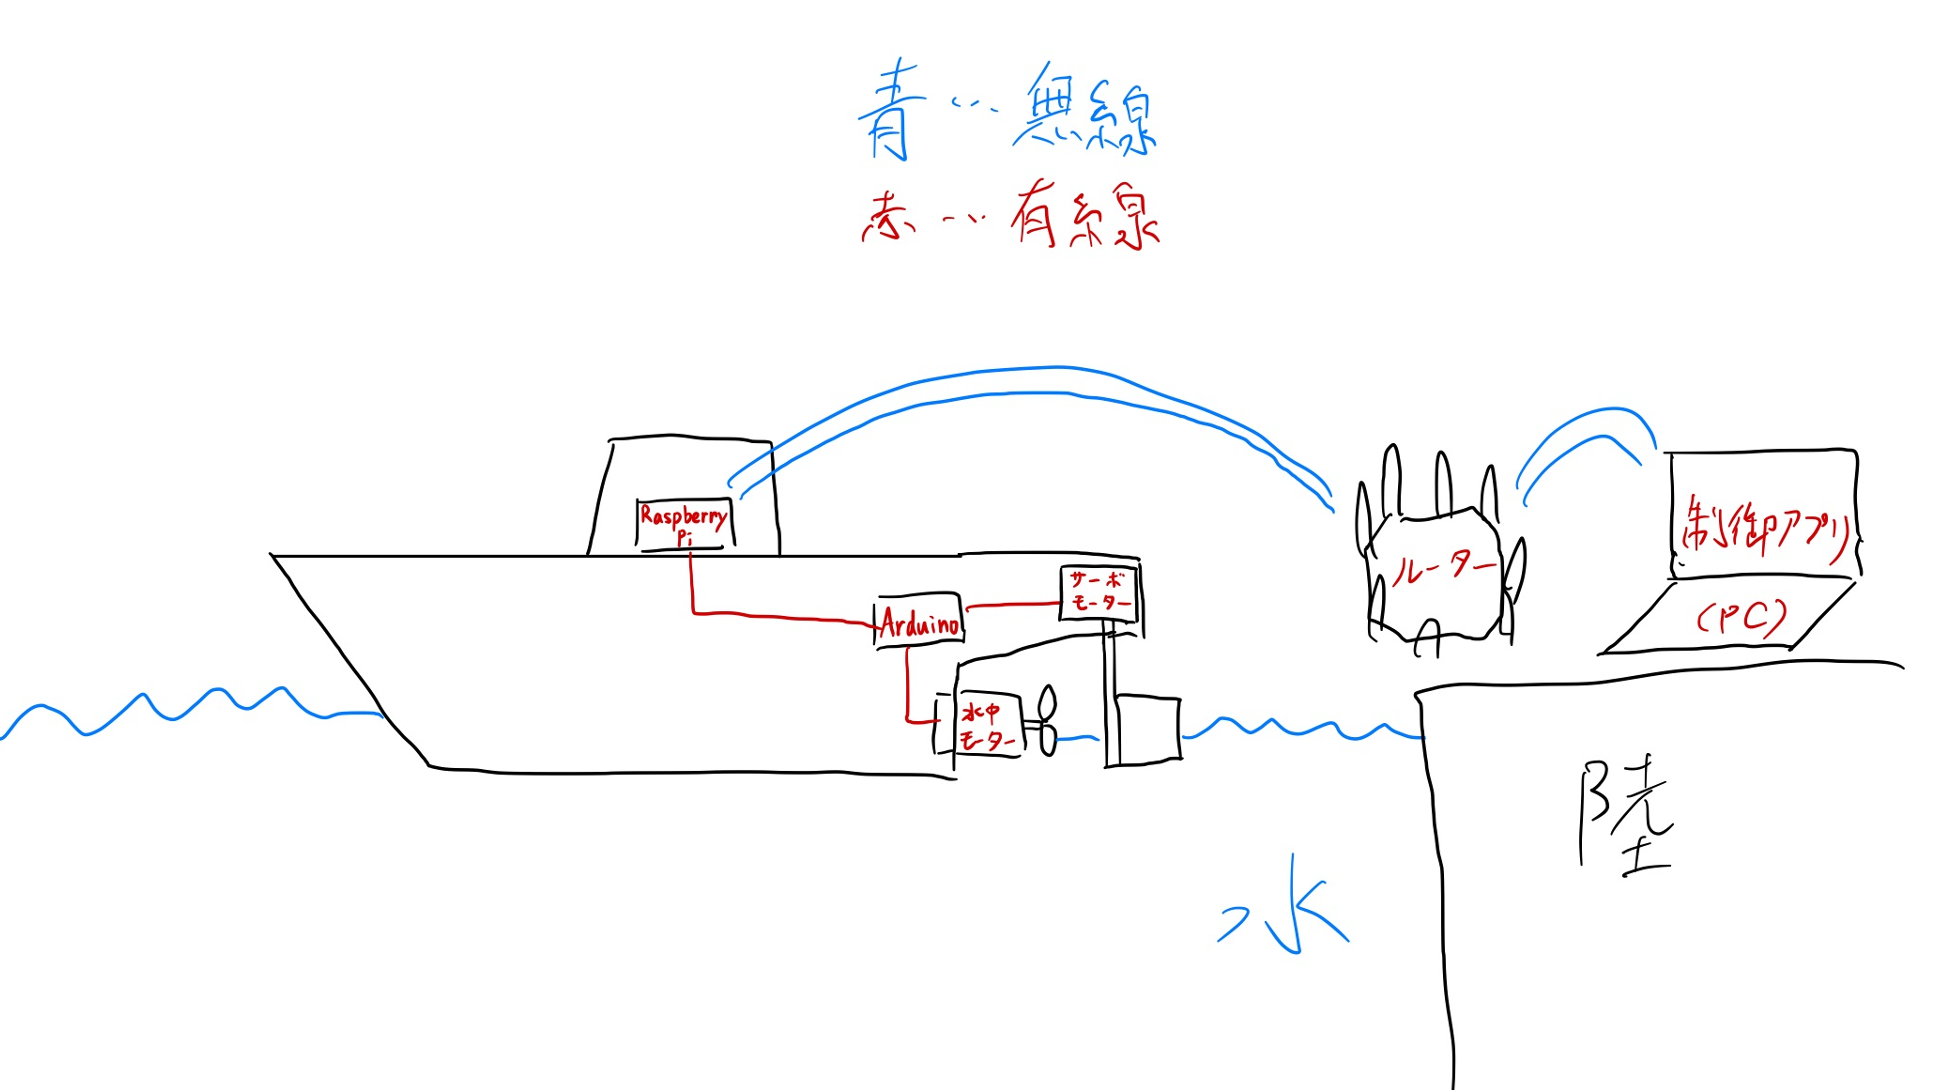
\includegraphics[width=100mm]{./remote_controller.png} 
\caption{通信の模式図}
\label{fugafuga}
\end{figure}

\begin{itemize}
  \item Arduino - モーター間
  Arduinoのコードは'ship/arduino-controller.ino'に入っています。
  ラジコン船にはブラシレスモーター2個と、サーボモーター1個を用いていて、そのためPWM(パルス幅変調)を使ってこれらのモーターを駆動しなければなりません。
  \item Raspberry Pi - Arduino間
  
  \item 制御用PC - ルーター - Raspberry Pi間
\end{itemize}
\subsubsection{設計(3Dモデリング)}

\subsubsection{その他}
ここでは完成した船を池に浮かべて実験する際の注意点や、これから加えていきたい機能について説明します。
\subsection{RACECAR}

\subsection{2進数計算機}

\section{反省点}
文化祭中ずっと朝の準備時間を他の参団(Apes Hunter)に費やしてしまい、その結果僕の作品のシフトの人に迷惑をかけてしまったようです...来年は物理部フルシフトで行くつもりなので、今後このようなことはないよう気をつけます。

\section{その他(ひとりごと)}
今年の文化祭で僕から提出した作品は、RACECARは中嶋幹(アメリカに留学中)と非物理部員の中野栄太郎君と、そして2進数計算機は中嶋君と作業して作りました。

そろそろChatGPTに頭が上がらない生活を脱却したいです...

\end{document}